\documentclass[tikz]{standalone}
\usepackage{tikz}
\usepackage{xcolor}

\usetikzlibrary{arrows.meta, positioning, shapes.multipart, calc, backgrounds}

\begin{document}
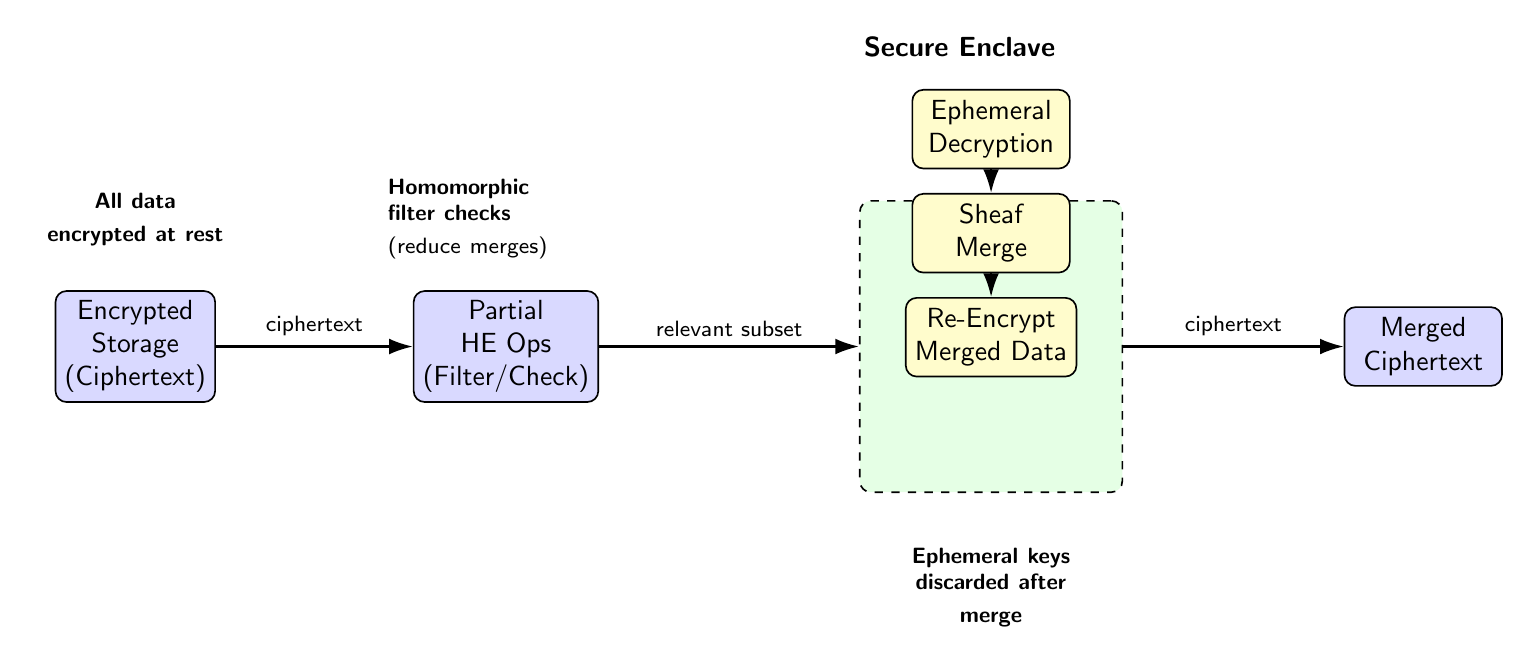
\begin{tikzpicture}[
    font=\sffamily,
    >=latex,
    line width=0.6pt,
    node distance=1.8cm and 2.5cm,
    box/.style={
      rectangle,
      draw,
      rounded corners,
      align=center,
      fill=blue!15,
      minimum width=2.0cm,
      minimum height=1.0cm
    },
    dashedbox/.style={
      rectangle,
      draw,
      dashed,
      rounded corners,
      align=center,
      fill=green!10,
      minimum width=2.5cm,
      minimum height=1.0cm
    },
    arrowstyle/.style={
      -{Latex[length=3mm, width=2mm]},
      line width=0.8pt
    }
]

% 1. NODES
\node[box] (storage) {Encrypted\\Storage\\(Ciphertext)};
\node[box, right=2.5cm of storage] (partialHE) {Partial\\HE Ops\\(Filter/Check)};
\node[dashedbox, right=3.3cm of partialHE, text width=3.1cm, minimum height=3.7cm, label={[xshift=-0.4cm,yshift=1.7cm]\textbf{Secure Enclave}}] (enclave) {};
\node[box, fill=yellow!20, yshift=0.9cm] at (enclave.north) (decrypt) {Ephemeral\\Decryption};
\node[box, fill=yellow!20, below=0.3cm of decrypt] (merge) {Sheaf\\Merge};
\node[box, fill=yellow!20, below=0.3cm of merge] (reencrypt) {Re-Encrypt\\Merged Data};

\node[box, right=2.8cm of enclave] (cipherout) {Merged\\Ciphertext};

% 2. ARROWS
\draw[arrowstyle] (storage) -- node[above]{\footnotesize ciphertext} (partialHE);
\draw[arrowstyle] (partialHE) -- node[above]{\footnotesize relevant subset} (enclave.west);

\draw[arrowstyle] (enclave.east) -- node[above]{\footnotesize ciphertext} (cipherout);

% Inside the enclave: flow from decrypt -> merge -> reencrypt
\draw[arrowstyle] (decrypt) -- (merge);
\draw[arrowstyle] (merge) -- (reencrypt);

% Add small notes or callouts
\node[align=center, text width=2.5cm] at ($(storage.north) + (0,0.9)$)
    {\footnotesize \textbf{All data}\\ \footnotesize \textbf{encrypted at rest}};

\node[align=left, text width=3.0cm] at ($(partialHE.north) + (0,0.9)$)
    {\footnotesize \textbf{Homomorphic}\\ \footnotesize \textbf{filter checks}\\ \footnotesize (reduce merges)};

\node[align=center, text width=2.3cm] at ($(enclave.south) + (0,-1.2)$)
    {\footnotesize \textbf{Ephemeral keys}\\ \footnotesize \textbf{discarded after}\\ \footnotesize \textbf{merge}};

\end{tikzpicture}
\end{document}
